%% LyX 2.0.2 created this file.  For more info, see http://www.lyx.org/.
%% Do not edit unless you really know what you are doing.
\documentclass[english]{beamer}
\usepackage[T1]{fontenc}
\usepackage[latin9]{inputenc}
\usepackage{listings}
\usepackage{color}
\usepackage{amsmath}
\usepackage{amssymb}
\usepackage{graphicx}

\makeatletter

%%%%%%%%%%%%%%%%%%%%%%%%%%%%%% LyX specific LaTeX commands.
%% Because html converters don't know tabularnewline
\providecommand{\tabularnewline}{\\}

%%%%%%%%%%%%%%%%%%%%%%%%%%%%%% Textclass specific LaTeX commands.
 % this default might be overridden by plain title style
 \newcommand\makebeamertitle{\frame{\maketitle}}%
 \AtBeginDocument{
   \let\origtableofcontents=\tableofcontents
   \def\tableofcontents{\@ifnextchar[{\origtableofcontents}{\gobbletableofcontents}}
   \def\gobbletableofcontents#1{\origtableofcontents}
 }
 \long\def\lyxframe#1{\@lyxframe#1\@lyxframestop}%
 \def\@lyxframe{\@ifnextchar<{\@@lyxframe}{\@@lyxframe<*>}}%
 \def\@@lyxframe<#1>{\@ifnextchar[{\@@@lyxframe<#1>}{\@@@lyxframe<#1>[]}}
 \def\@@@lyxframe<#1>[{\@ifnextchar<{\@@@@@lyxframe<#1>[}{\@@@@lyxframe<#1>[<*>][}}
 \def\@@@@@lyxframe<#1>[#2]{\@ifnextchar[{\@@@@lyxframe<#1>[#2]}{\@@@@lyxframe<#1>[#2][]}}
 \long\def\@@@@lyxframe<#1>[#2][#3]#4\@lyxframestop#5\lyxframeend{%
   \frame<#1>[#2][#3]{\frametitle{#4}#5}}
 \def\lyxframeend{} % In case there is a superfluous frame end

%%%%%%%%%%%%%%%%%%%%%%%%%%%%%% User specified LaTeX commands.
\usepackage{listings}
\usetheme{Warsaw}
% or ...
%\usetheme{Antibes}	% tree outline, neat
%\usetheme{JuanLesPins}	% like Antibes, with shading
%\usetheme{Bergen}	% outline on side
%\usetheme{Luebeck}	% like Warsaw, square sides
%\usetheme{Berkeley}	% interesting left bar outline
%\usetheme{Madrid}	% clean, nice.  7/12 page numbers
%\usetheme{Berlin}	% dots show slide number
%\usetheme{Malmoe}	% OK, plain, unshaded
%\usetheme{Boadilla}	% nice, white bg, no top bar
%\usetheme{Marburg}	% nice, outline on right
%\usetheme{boxes}	% ???
%\usetheme{Montpellier}	% tree outline on top, plainish white
%\usetheme{Copenhagen}	% like Warsaw
%\usetheme{PaloAlto}	% looks good
%\usetheme{Darmstadt}	% like Warsaw with circle outline
%\usetheme{Pittsburgh}
%\usetheme{default}
%\usetheme{Rochester}	% like boxy, unshaded warsaw
%\usetheme{Dresden}	% circle outline on top
%\usetheme{Singapore}	% purple gradient top
%\usetheme{Frankfurt}	% like Warsaw with circle outline on top
%\usetheme{Szeged}
%\usetheme{Goettingen}	% light purple right bar outline
%\usetheme{Warsaw}
%\usetheme{Hannover}	% like Goett with bar on left
%\usetheme{compatibility}
%\usetheme{Ilmenau}

\setbeamercovered{transparent}
% or whatever (possibly just delete it)

%\usecolortheme{seahorse}
%\usecolortheme{rose}

% seems to fix typewriter font in outline header:
\usepackage{ae,aecompl}

\usepackage[toc]{multitoc}

\makeatother

\usepackage{babel}
\begin{document}

\title[Firebase Security 2.0]{Firebase Security 2.0:}


\subtitle{A Sm�rg�sbord of evolutionary and revolutionary changes for your
consideration}


\author[Tom Larkworthy]{Tom Larkworthy\\}


\date{Wed 9th, 2014}

\makebeamertitle
\pgfdeclareimage[height=0.5cm]{institution-logo}{institution-logo-filenameO}

\logo{\pgfuseimage{institution-logo}}

% RPD:  can't get this to work on any template.  not present in Warsaw any way, it seems

% hmm, problem seems to be that it isn't copied to the tmp dir, probably becuase it doesn't have the

% filename extension (which is tacked on by pgf it seems)

%\AtBeginSubsection[]{

%  \frame<beamer>{ 

%    \frametitle{Outline}   

%    \tableofcontents[currentsection,currentsubsection] 

%  }

%}

%\beamerdefaultoverlayspecification{<+->}


\lyxframeend{}\lyxframe{Outline}

\begin{multicols}{2}

\tableofcontents{}

\end{multicols}


\lyxframeend{}


\lyxframeend{}\lyxframe{Critique of Existing Rules}
\begin{itemize}
\item Syntax
\item quotes and comma and fiddly

\begin{itemize}
\item no comments or multi-line string in JSON
\end{itemize}
\item Reuse

\begin{itemize}
\item of model classes for denormalization
\item of common phrases in rules
\end{itemize}
\item Semantics

\begin{itemize}
\item write: false ... allows writes if child overrides
\item mix of concerns, access control, integrity constrains and schema
\end{itemize}
\item Extendability
\item Testing is hard work
\end{itemize}

\lyxframeend{}


\lyxframeend{}\section{Language}


\lyxframeend{}\subsection{Basic YAML}


\lyxframeend{}\lyxframe{\texttt{Basic YAML}}
\begin{itemize}
\item YAML superset of JSON
\item comments, unquoted keys, unquotes strings, multi-line strings, no
commas
\item indentation if not using JSON syntax\end{itemize}
\begin{block}
{\scriptsize \lstinputlisting{basic_yaml.yaml}}{\scriptsize \par}
\end{block}

\lyxframeend{}


\lyxframeend{}\subsection{YAML to JSON}


\lyxframeend{}\lyxframe{\texttt{YAML $\rightarrow$ JSON}}
\begin{itemize}
\item trivial transformation, pure JS implementation, js-yaml for node,
CLI or Browser
\item suggestions: display documentation in YAML and JSON?\end{itemize}
\begin{block}
{\scriptsize \lstinputlisting{basic_yaml.json}}{\scriptsize \par}
\end{block}

\lyxframeend{}


\lyxframeend{}\subsection{Advanced YAML}


\lyxframeend{}\lyxframe{\texttt{Advanced YAML}}
\begin{itemize}
\item block string literals, $>$
\item merge keys operator, $<<$
\item anchor and reference, $\&$ and $*$
\item source maps (not available, but column and row tracked in js-yaml)\end{itemize}
\begin{block}
{\scriptsize \lstinputlisting{advanced_yaml.yaml}}{\scriptsize \par}
\end{block}

\lyxframeend{}


\lyxframeend{}\lyxframe{\texttt{Advanced YAML}}
\begin{block}
{\scriptsize \lstinputlisting{advanced_yaml.json}}{\scriptsize \par}
\end{block}

\lyxframeend{}


\lyxframeend{}\subsection{Summery}


\lyxframeend{}\lyxframe{YAML Summery}
\begin{itemize}
\item well known (esp. python or ruby or GAE)
\item solves all current syntax wrinkles
\item easy to read
\item ugly, but functional reuse
\item Entire spec is massive but dedicated to types, many implementations
do not support all of it

\begin{itemize}
\item !!js/function
\end{itemize}
\item Internally everything is JSON, but write the front end YAML (or write
in JSON if you prefer). 
\end{itemize}

\lyxframeend{}


\lyxframeend{}\section{Security Expressions}


\lyxframeend{}\subsection{Rule Variables}


\lyxframeend{}\lyxframe{Rule Variables}

\begin{tabular}{c|c|c|c|cc}
\cline{1-5} 
old names & data & newData & root & (newRoot) & \tabularnewline
\hline 
\hline 
temporal & before & after &  &  & \tabularnewline
\cline{1-5} 
 & \textcolor{green}{prev} & \textcolor{green}{next} &  & root\_next & same length\tabularnewline
\cline{1-5} 
 &  & nxt &  &  & \tabularnewline
\multicolumn{1}{c}{} & \multicolumn{1}{c}{} & \multicolumn{1}{c}{} & \multicolumn{1}{c}{} &  & \tabularnewline
\hline 
client/server & \textcolor{red}{ref} & \textcolor{red}{req} &  &  & like client API\tabularnewline
\cline{1-5} 
 & db & cursor &  &  & \tabularnewline
\cline{1-5} 
 & server & client &  &  & \tabularnewline
\cline{1-5} 
 &  & in &  &  & \tabularnewline
\cline{1-5} 
 &  & usr &  &  & \tabularnewline
\end{tabular}


\lyxframeend{}


\lyxframeend{}\subsection{Predicates}


\lyxframeend{}\lyxframe{Rule Predicates}
\begin{itemize}
\item Boolean functions: $x\mapsto\mathbb{B}$
\item Encode the function declaration in the key

\begin{itemize}
\item prevents users defining a procedural body
\end{itemize}
\end{itemize}
\begin{block}
{\scriptsize \lstinputlisting{predicates.yaml}}{\scriptsize \par}
\end{block}

\lyxframeend{}


\lyxframeend{}


\lyxframeend{}\subsection{Dereferencing}


\lyxframeend{}\lyxframe{Child Dereferencing}
\begin{block}
{\scriptsize \lstinputlisting{dereferencing.yaml}}{\scriptsize \par}
\end{block}

\lyxframeend{}


\lyxframeend{}\section{Schema}


\lyxframeend{}\lyxframe{What is Schema?}
\begin{itemize}
\item The static structure
\item the integrity constraints
\item JSON Schema, YAML, Finitio (was Q)
\item \textbf{Not} the access permissions
\end{itemize}

\lyxframeend{}


\lyxframeend{}\subsection{JSON Schema}


\lyxframeend{}\lyxframe{JSON Schema (in YAML)}
\begin{block}
{\scriptsize \lstinputlisting{person.yaml}}{\scriptsize \par}
\end{block}

\lyxframeend{}


\lyxframeend{}\lyxframe{Inheritance}
\begin{block}
{\scriptsize \lstinputlisting{polygon.yaml}}{\scriptsize \par}
\end{block}

\lyxframeend{}


\lyxframeend{}\subsection{\$ Wildcards}


\lyxframeend{}\lyxframe{\$vars}
\begin{itemize}
\item wildcards are supported out-of-the-box through regex matching
\item but named groups are verbose to bind the match, so we should facade
patternProperties\end{itemize}
\begin{block}
{\scriptsize \lstinputlisting{wildcards.yaml}}{\scriptsize \par}
\end{block}

\lyxframeend{}


\lyxframeend{}\subsection{Constraints}


\lyxframeend{}\lyxframe{Integrity Constraints}
\begin{itemize}
\item ALL global constraints must evaluate to true to write, NO inheritance\end{itemize}
\begin{block}
{\scriptsize \lstinputlisting{constraints.yaml}}{\scriptsize \par}
\end{block}

\lyxframeend{}


\lyxframeend{}\subsection{Access Control}


\lyxframeend{}\lyxframe{Access Control}
\begin{block}
{\scriptsize \lstinputlisting{acl.yaml}}{\scriptsize \par}\end{block}
\begin{itemize}
\item Obvious place for triggers
\item Would be nice to override predicates here too if possible
\end{itemize}

\lyxframeend{}


\lyxframeend{}\subsection{Meta Schema}


\lyxframeend{}\lyxframe{Meta Schema}

\begin{center}
\begin{tabular}{|c|c|c|}
\hline 
level & schema & language\tabularnewline
\hline 
\hline 
data & user-schema & JSON\tabularnewline
\hline 
user-schema & meta-schema & JSON\tabularnewline
\hline 
meta-schema & meta-schema & JSON\tabularnewline
\hline 
\end{tabular}
\par\end{center}
\begin{itemize}
\item What constitutes a valid user-schema is described by the meta-schema
(which is also a valid schema!)
\item The meta-schema states the allowed keywords, e.g. ``type'' or ``properties''
\end{itemize}



\lyxframeend{}


\lyxframeend{}\lyxframe{JSON Schema's meta-schema}
\begin{block}
{\scriptsize \lstinputlisting{meta-schema.yaml}}{\scriptsize \par}
\end{block}

\lyxframeend{}


\lyxframeend{}\lyxframe{ADT}
\begin{itemize}
\item Meaningful keywords are created by extending the meta-schema (e.g.
constraint)
\item Keywords affect how security rules are generated (e.g. require)
\item Existing keywords have to affect the rules anyway (e.g. additionProperties
= false)
\item The validity of a keyword is dependent on type (e.g. minimum)
\item So bottom up traverse the schema tree, looking at the ``type''
\end{itemize}

\lyxframeend{}


\lyxframeend{}\lyxframe{Queue}
\begin{block}
{\scriptsize \lstinputlisting{queue.yaml}}{\scriptsize \par}
\end{block}

\lyxframeend{}


\lyxframeend{}\lyxframe{Queue}
\begin{block}
{\scriptsize \lstinputlisting{queue.yaml}}{\scriptsize \par}
\end{block}

\lyxframeend{}


\lyxframeend{}\lyxframe{Meta-schema}
\begin{itemize}
\item The same mechanism can be used to decide how ``minimum'' gets mapped
into constraints
\item As schema are URL references, you can import other peoples ADTs!
\end{itemize}

\lyxframeend{}


\lyxframeend{}\lyxframe{VM}
\begin{itemize}
\item What about a VM for a ADT to verify a user has run some byte code
correctly

\begin{itemize}
\item cross compile C++ to Firebase for serverside verification
\item missing >\textcompwordmark{}> and >\textcompwordmark{}>\textcompwordmark{}>
bitwise operators \& |
\end{itemize}
\item explicitly represent the VM state (program counter, program, registers,
memory)
\item Client steps through bytecode like a debugger

\begin{itemize}
\item server notifies client only if desyncs
\item client gets results before the server is aware!
\item server can be sure client has run the correct code!
\end{itemize}
\end{itemize}

\lyxframeend{}


\lyxframeend{}\subsection{Initial Firebase}


\lyxframeend{}\lyxframe{Initial Firebase}
\begin{block}
{\scriptsize \lstinputlisting{noob.yaml}}{\scriptsize \par}\end{block}
\begin{itemize}
\item would be nice to one click to a basic template, e.g. federated users
\end{itemize}

\lyxframeend{}


\lyxframeend{}\subsection{JSON Schema Ecosystem }


\lyxframeend{}\lyxframe{JSON Schema adoption}

\begin{center}
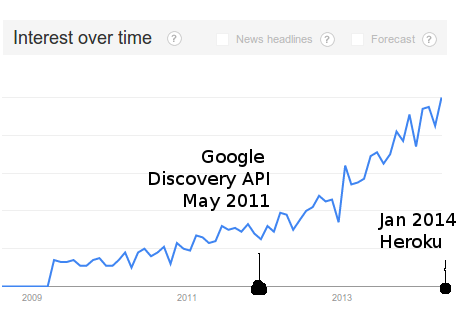
\includegraphics[width=6cm]{json_schema_trends}
\par\end{center}
\begin{itemize}
\item IETF draft v4, v5 fixes unioned meta-schema with control flow statements.
v5 is last draft
\item v1-3 written by different people than v4 onwards
\end{itemize}

\lyxframeend{}


\lyxframeend{}\lyxframe{Tooling}
\begin{itemize}
\item existing documentation on how to write JSON schema
\item Validators in every language
\item Hyper-schema describes the REST interface (which contains schema)
\item Heroku clients (ruby, scala, node) dynamically generate clients from
hyper-schema
\item static code generators not mature
\item UI generation from Hyper-schema
\item documentation generation
\item \textit{interoperability}
\end{itemize}

\lyxframeend{}


\lyxframeend{}\lyxframe{JSON-editor}

\begin{center}
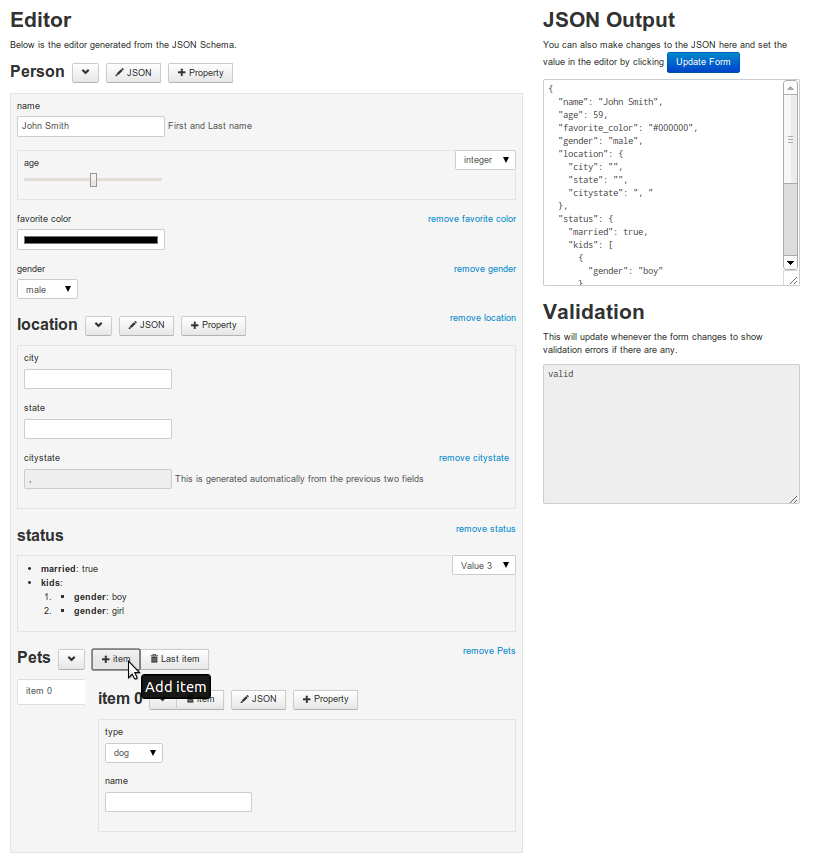
\includegraphics[width=8cm]{json-editor}
\par\end{center}


\lyxframeend{}


\lyxframeend{}\lyxframe{JSON Schema Good bits}
\begin{itemize}
\item \$ref (\& and {*} in YAML)
\item required
\item additionProperties = false
\item enum
\item allOf ( merge key in YAML)
\item properties
\item type
\end{itemize}

\lyxframeend{}


\lyxframeend{}\section{Testing}


\lyxframeend{}\subsection{inline}


\lyxframeend{}\lyxframe{Testing}
\begin{itemize}
\item development of schema/rules is error prone
\item inline tests can catch semantic errors at ``compile'' time\end{itemize}
\begin{block}
{\scriptsize \lstinputlisting{testing.yaml}}{\scriptsize \par}
\end{block}

\lyxframeend{}


\lyxframeend{}\subsection{CTL}


\lyxframeend{}\lyxframe{Verification}
\begin{itemize}
\item Dynamic behavior of database even harder to predict
\item Computational Tree Logic (CTL) is a formal language for describing
temporal evolution of logical systems

\begin{itemize}
\item $\mathbf{A}$ means all paths
\item $\mathbf{\mathbf{E}}$ means there exists a path
\item $\mathbf{G}$ global modifier (always true)
\item $\mathbf{F}$ finally modifier (the path leads to ...)
\end{itemize}
\item SPEC AG EF users.fred.state = IDLE
\item SPEC !EF (users.john.item = gold \& users.fred.item = gold)
\end{itemize}

\lyxframeend{}


\lyxframeend{}\lyxframe{Verification}
\begin{block}
{\scriptsize \lstinputlisting{specs.yaml}}{\scriptsize \par}
\end{block}

\lyxframeend{}


\lyxframeend{}\section{Suggestions List}


\lyxframeend{}\lyxframe{Suggestions}

\begin{center}
{\footnotesize }%
\begin{tabular}{|c|c|c|c|c|c|}
\hline 
{\footnotesize domain} & {\footnotesize suggestion} & {\footnotesize implications} & {\footnotesize hard?} & {\footnotesize USP?} & {\footnotesize TAM}\tabularnewline
\hline 
\hline 
{\footnotesize language} & {\footnotesize use YAML} & {\footnotesize convertion step} & {\footnotesize 1} & {\footnotesize 2} & {\footnotesize 100\%}\tabularnewline
\cline{2-6} 
 & {\footnotesize support YAML/JSON} & {\footnotesize website bifocal} & {\footnotesize 2} & {\footnotesize 1} & {\footnotesize 60\%}\tabularnewline
\cline{3-6} 
 &  & {\footnotesize source maps} & {\footnotesize 2} & {\footnotesize 2} & {\footnotesize 100\%}\tabularnewline
\hline 
\hline 
{\footnotesize security expr.} & {\footnotesize change newData} &  & {\footnotesize 1} & {\footnotesize 1} & {\footnotesize 100\%}\tabularnewline
\cline{2-6} 
 & {\footnotesize predicates} & {\footnotesize parsing key} & {\footnotesize 2} & {\footnotesize 2} & {\footnotesize 80\%}\tabularnewline
\cline{3-6} 
 &  & {\footnotesize scoping} & {\footnotesize 3} & {\footnotesize 1} & {\footnotesize 50\%}\tabularnewline
\cline{2-6} 
 & {\footnotesize dereferencing} & {\footnotesize API clashes} & {\footnotesize 1} & {\footnotesize 2} & {\footnotesize 90\%}\tabularnewline
\cline{2-6} 
 & {\footnotesize update docs} &  & {\footnotesize 2} & {\footnotesize 1} & {\footnotesize 75\%}\tabularnewline
\hline 
\end{tabular}
\par\end{center}{\footnotesize \par}


\lyxframeend{}


\lyxframeend{}\lyxframe{{\footnotesize Suggestions}}

\begin{center}
{\footnotesize }%
\begin{tabular}{|c|c|c|c|c|c|}
\hline 
{\footnotesize domain} & {\footnotesize suggestion} & {\footnotesize implications} & {\footnotesize hard?} & {\footnotesize USP?} & {\footnotesize TAM}\tabularnewline
\hline 
\hline 
{\footnotesize schema} & {\footnotesize support v4} & {\footnotesize expr. generation} & {\footnotesize 5} & {\footnotesize 3} & {\footnotesize 90\%}\tabularnewline
\cline{2-6} 
 & {\footnotesize meta-schema} & {\footnotesize extendability} & {\footnotesize 5} & {\footnotesize 4} & {\footnotesize 40\%}\tabularnewline
\cline{3-6} 
 &  & {\footnotesize VM} & {\footnotesize 9} & {\footnotesize 10} & {\footnotesize 3\%}\tabularnewline
\cline{2-6} 
 & {\footnotesize ACL} & {\footnotesize expr. generation} & {\footnotesize 4} & {\footnotesize 2} & {\footnotesize 100\%}\tabularnewline
\cline{3-6} 
 &  & {\footnotesize triggers} & {\footnotesize 1} & {\footnotesize 2} & {\footnotesize 60\%}\tabularnewline
\cline{2-6} 
 & {\footnotesize hyper schema serving} & {\footnotesize hosting integration} & {\footnotesize 3} & {\footnotesize 4} & {\footnotesize 40\%}\tabularnewline
\cline{3-6} 
 &  & {\footnotesize UI generation} & {\footnotesize 3} & {\footnotesize 4} & {\footnotesize 50\%}\tabularnewline
\hline 
{\footnotesize Testing} & {\footnotesize inline (non) examples} & {\footnotesize example} & {\footnotesize 1} & {\footnotesize 3} & {\footnotesize 40\%}\tabularnewline
\cline{2-6} 
 & {\footnotesize CTL} & {\footnotesize serverside processing} & {\footnotesize 10} & {\footnotesize 10} & {\footnotesize 5\%}\tabularnewline
\cline{3-6} 
 &  & {\footnotesize new billing} & {\footnotesize 6} & {\footnotesize 1} & {\footnotesize 5\%}\tabularnewline
\hline 
\end{tabular}
\par\end{center}{\footnotesize \par}


\lyxframeend{}
\end{document}
